\chapter{Tasks of the project}
\section{Task Identification}
The project is composed of the following tasks:

\begin{table}[H]
	\centering
	\begin{tabular}{ r l } 
		\textbf{RASD} & T1: Requirement Specification \\
					  & T2: UML Diagrams \\
			          & T3: Alloy Model \\
		\textbf{DD} & T4: Architectural Design \\
					& T5: Algorithm Design \\
					& T6: Requirement Traceability \\
		\textbf{ITPD} & T7: ITPD \\
		\textbf{PM} & T8: FP \\
					& T9: COCOMO \\
					& T10: Task Identification \\
					& T11: Resources Allocation \\
					& T12: Risk Management \\
		\textbf{PRESENTATION} & T13: Presentation \\
		\textbf{DEVELOPMENT} & T14: Development \\
		\textbf{TESTING} & T15: Unit Testing \\
						 & T16: Integration Testing
	\end{tabular}
\end{table}

\section{Gantt Diagram}

\begin{figure}[H]
	\centering
	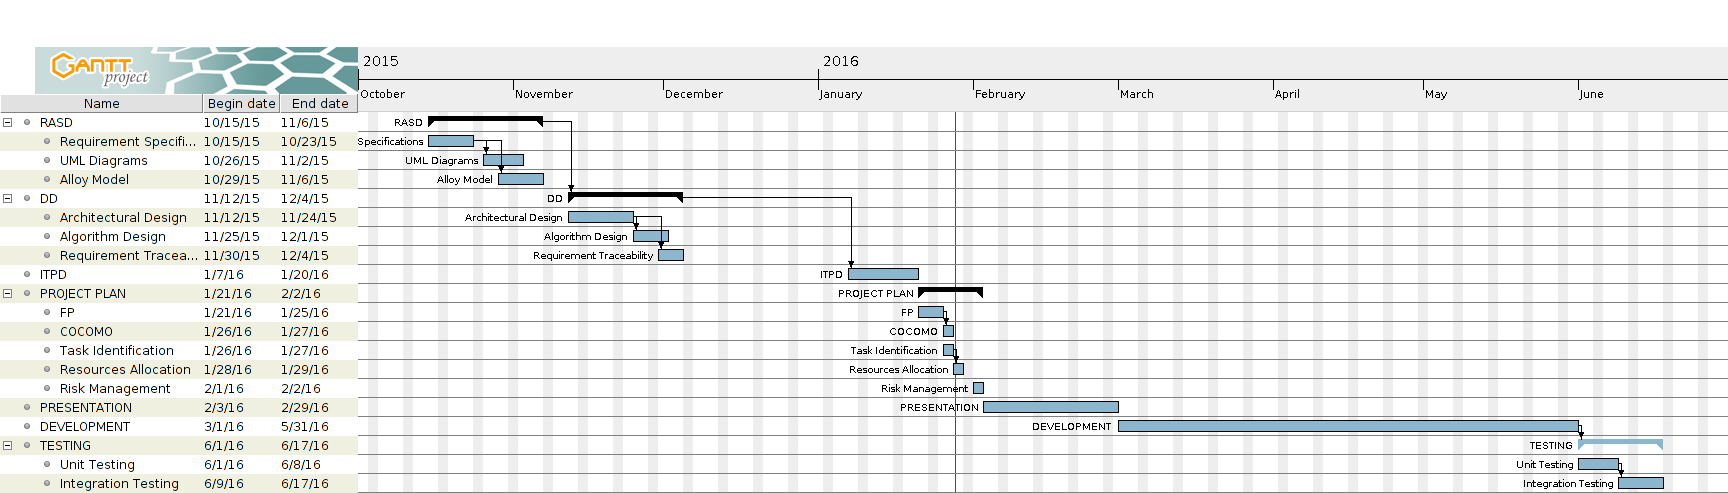
\includegraphics[angle=90,scale=0.4]{Tasks/gantt}
\end{figure}
